\section{Theoretical Analysis}
\label{sec:analysis}

In this section, the circuit shown in Figure~\ref{fig:circuit_t1} is analysed
theoretically using two methods: the mesh analysis and the nodal anaylis.\par
For the mesh analysis 4 variables were created - the 4 mesh currents.{\it$I_{SE}$ } is the mesh current of the mesh on the top left corner of our circuit (clockwise). {\it$I_{SD}$}is the mesh current of the mesh on the top right corner of our circuit (counter clockwise).{\it$I_{IE}$ } is the mesh current of the mesh on the lower left corner of our circuit(counter clockwise). {\it$I_{ID}$} is the mesh current of the mesh on the lower right corner of our circuit(counter clockwise).Knowing the mesh currents, and using Ohm's law we can determine any node voltage or branch current. To determine the 4 unknown mesh currents we used the following 4 equations.


\input{mesh_eq_tab}

With the help of Octave, the equations yielded the following values for the mesh currents.(********************adicionar tabela?**************************)\par

For the nodal analysis we apply the Kirchhoff Current Law (KCL) to the nodes that are not conected to voltage sources (equations 7 to 11). We obtain 2 more equations from the potencial difference at the terminals of the voltage sources (equations 12 and 13).As it was stated before, node 0 is the ground node and therefore the voltage at this node is 0V (equation 1). For the simulation analysis it was necessesary to add an other "fictional" voltage source that provides 0 volts to the circuit, between node 7 and resistor 6. This "fictional" voltage source was also considered in the Theoretical Analysis, as it has no real effect on the circuit. This yiels equation number 6. Now we have 9 equations for 9 unkown variables- voltage ({\it$V_{0}$}  to {\it$V_{8}$}.Using Octave we determine the values of every node voltage of the circuit. \par

\input{nodal_eq_tab}

%\begin{figure}[h] \centering
%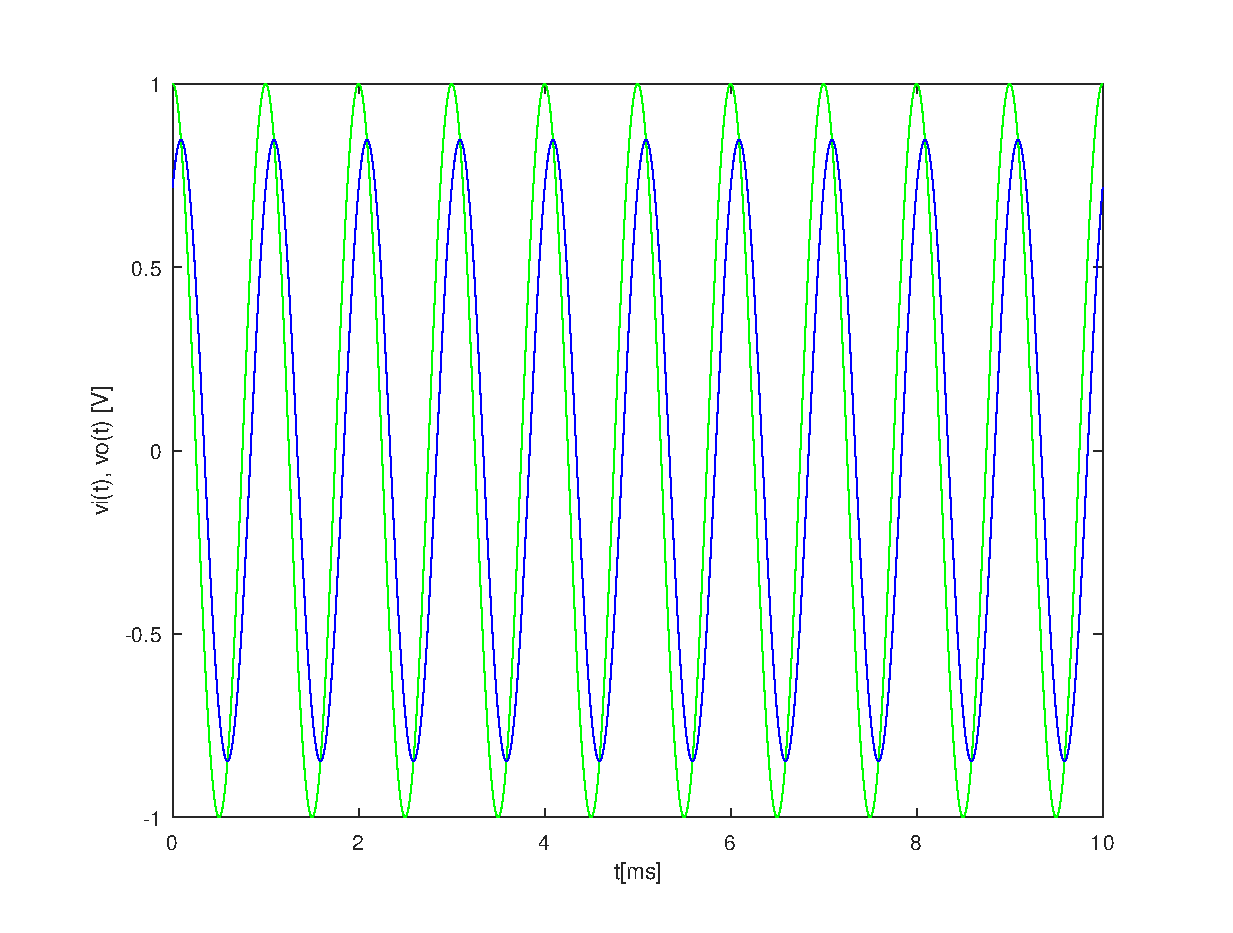
\includegraphics[width=0.8\linewidth]{forced.eps}
%\caption{Forced sinusoidal response.}
%\label{fig:forced}
%\end{figure}


In Table~\ref{tab:theoretical} the values for the branch currents and the node voltages obtained from the ocatve script for both methods are presented.\par 
\begin{table}[h]
  \centering
  \begin{tabular}{|l|r|r|}
    \hline    
    {\bf Name} & {\bf Mesh method} & {\bf Node method}\\ \hline
    @Gb & -0.291567 & -0.291567 \\ \hline
@id & 1.018915 & 1.018915 \\ \hline
@r1 & -0.278049 & -0.278049 \\ \hline
@r2 & -0.291567 & -0.291567 \\ \hline
@r3 & -0.013518 & -0.013518 \\ \hline
@r4 & 1.226887 & 1.226887 \\ \hline
@r5 & 1.310482 & 1.310482 \\ \hline
@r6 & -0.948838 & -0.948838 \\ \hline
@r7 & -0.948838 & -0.948838 \\ \hline
V1 & 5.243596 & 5.243596 \\ \hline
V2 & 4.952740 & 4.952740 \\ \hline
V3 & 4.367469 & 4.367469 \\ \hline
V4 & 4.994112 & 4.994112 \\ \hline
V5 & 9.086122 & 9.086122 \\ \hline
V6 & -2.926767 & -2.926767 \\ \hline
V7 & -1.963402 & -1.963402 \\ \hline
V8 & -1.963402 & -1.963402 \\ \hline

  \end{tabular}
  \caption{A variable preceded by @ is of type {\em current}
    and expressed in milliampere (mA); other variables are of type {\it voltage} and expressed in
    Volt (V).}
  \label{tab:theoretical}
\end{table}

As it can be seen this values are the same, which suggests that for these simple circuit, the methods are equally precise. 
